\documentclass[tesis.tex]{subfiles}

\begin{document}
    
\section{Methods}

\subsection{Field observations}

Four field campaigns were carried out between 2010 and 2012 described in the work of \cite{Williams2014} and \cite{williams2016}, but in this work, we will focus exclusively on the data between January and March 2012 to analyze the behavior of the estuary in a closed state. Measurements were made using instruments for speed and depth, as well as including a meteorological station to collect wind speed and direction data. Depth data were collected using moored pressure, conductivity, and temperature sensors (CTD) placed at different heights and distributed along the estuary at four points as shown in (Fig. \ref{fig:mapPDO}), called Near Mouth (NM), Mid-Lagoon (ML), Deep Channel (DC), and Pescadero Creek (PC). Density profiles were made on February 16th with a CTD logger around 5 p.m. at the locations indicated in Fig. \ref{fig:mapPDO}. The moment the profiles were made the wind was calm, so is not causing a disturbance in the water.


\begin{figure}[h!]
    \centering
    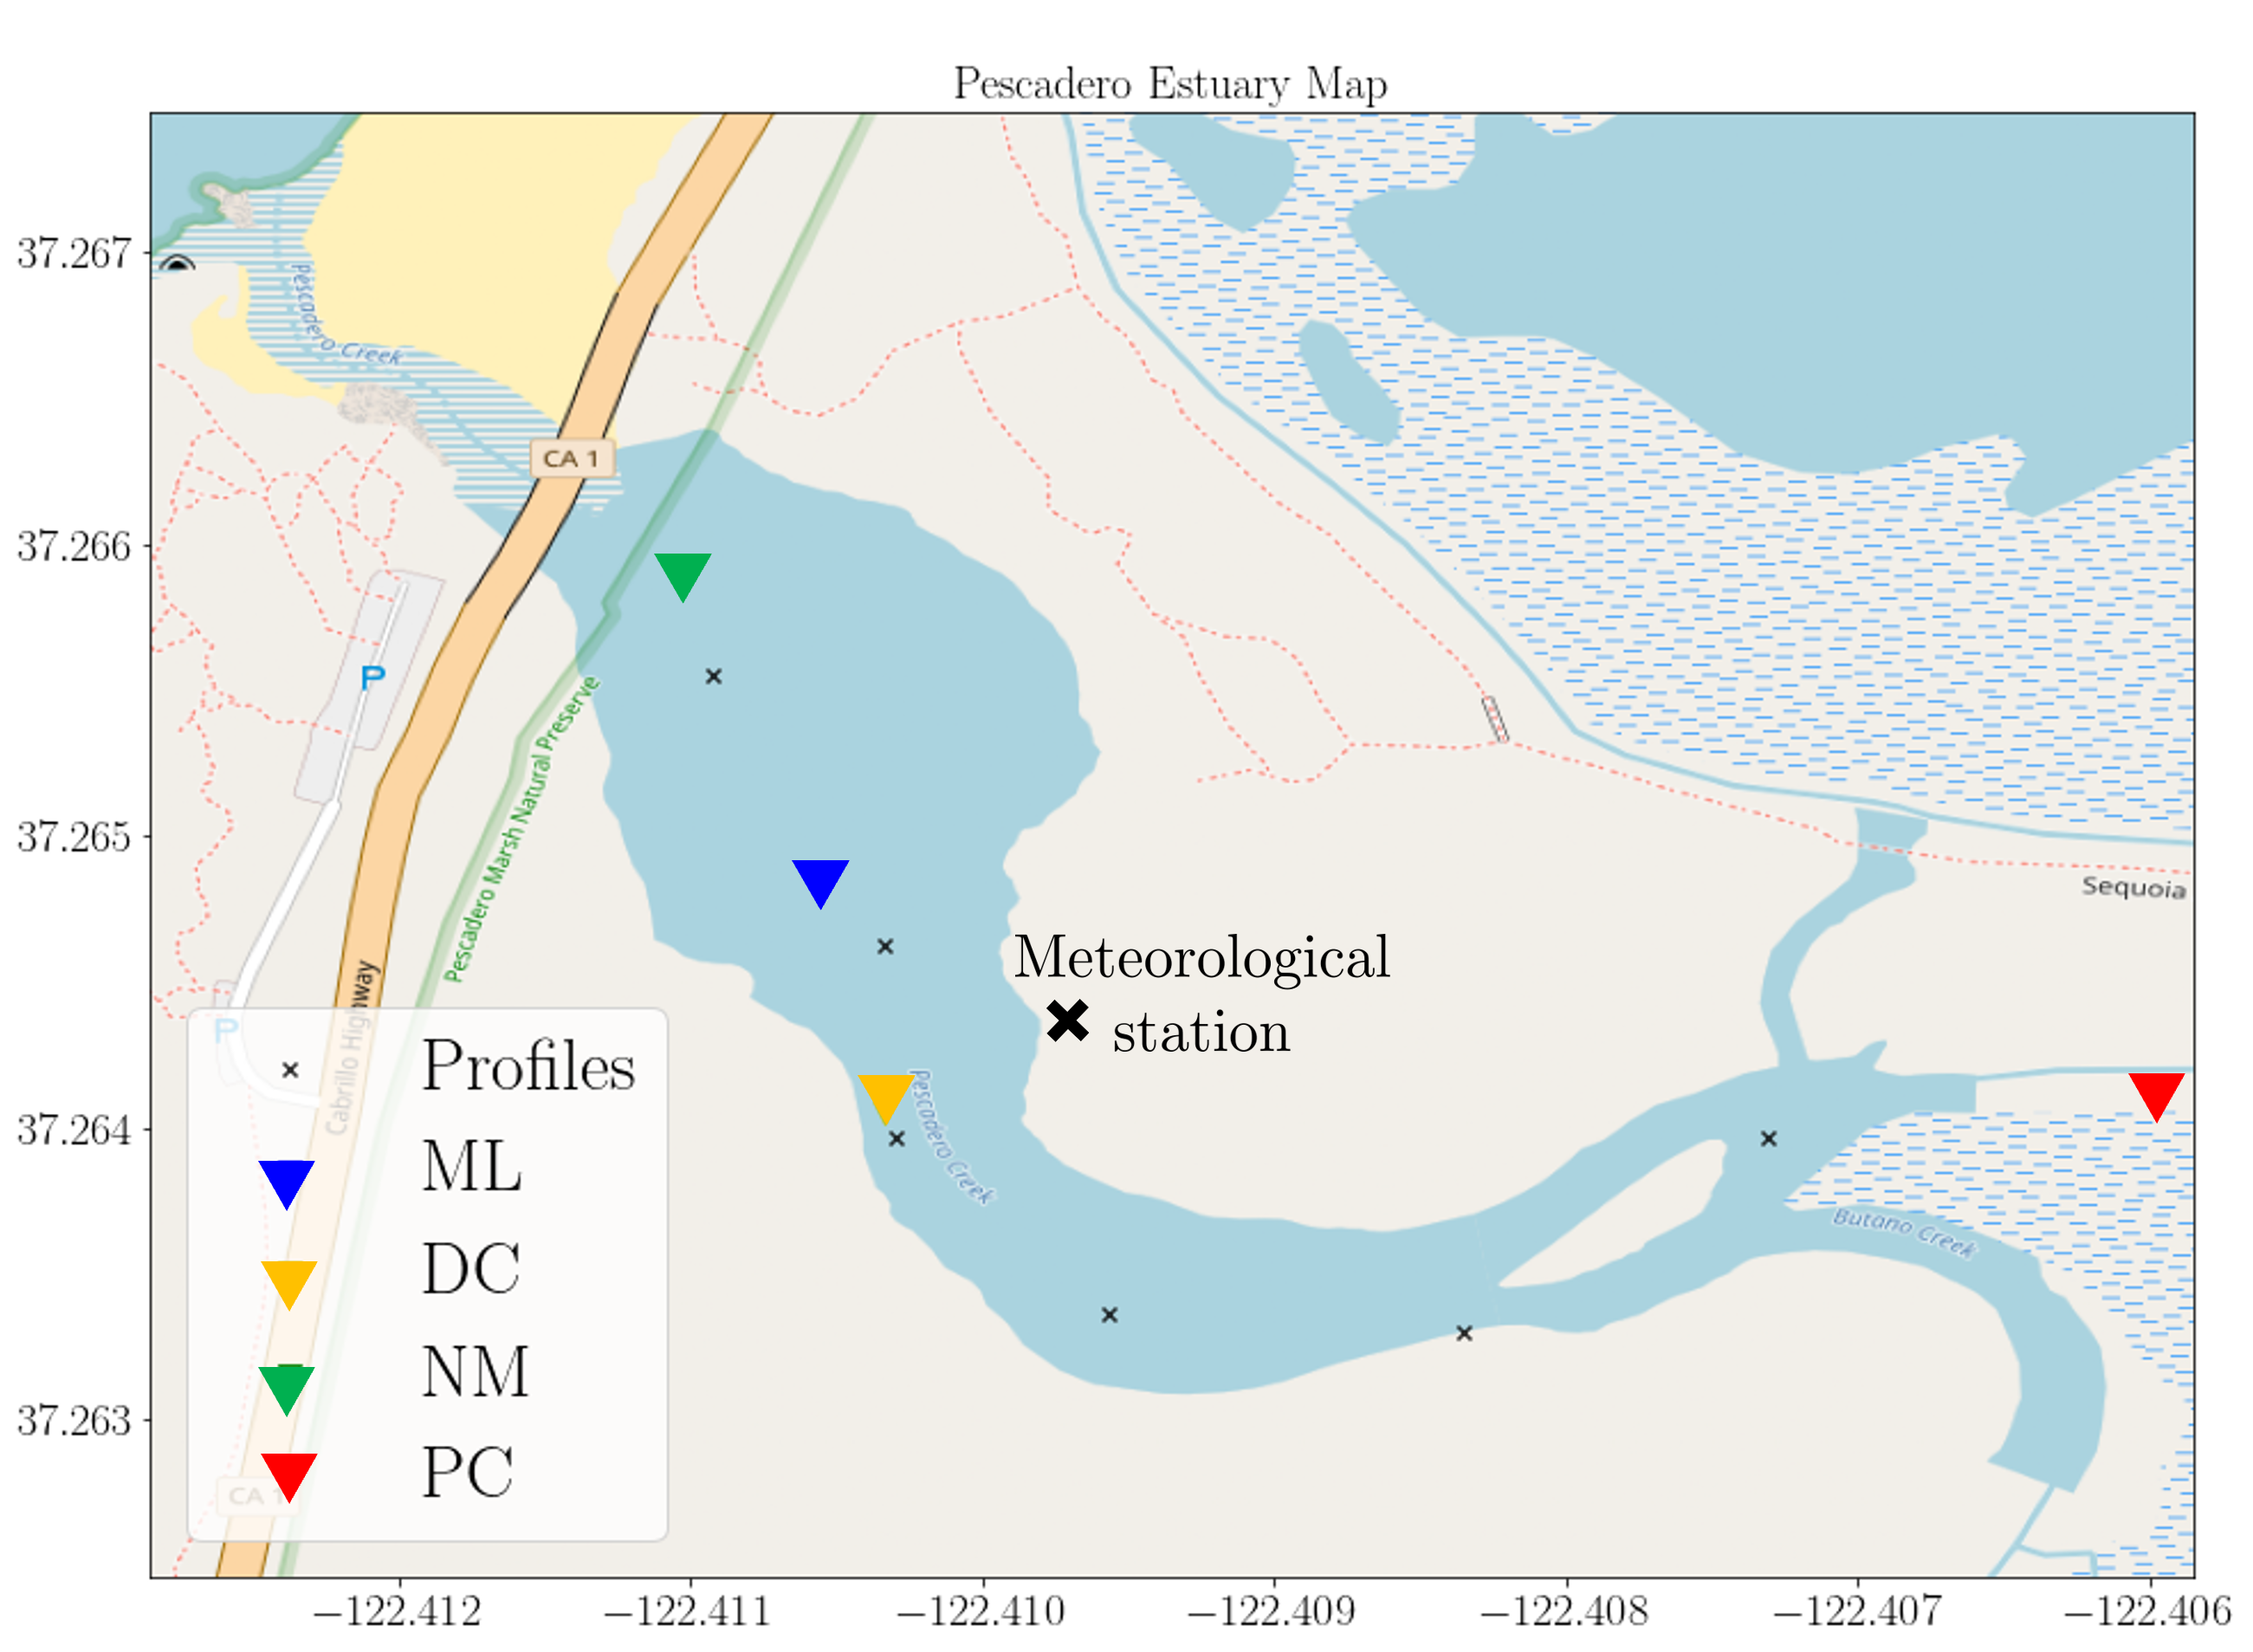
\includegraphics[scale=0.6]{Imagenes/mapa2.png}
    \caption{Pescadero estuary map and location of the sensors (NM: Near Mouth, ML: Mid-Lagoon, DC: Deep Channel and, PC: Pescadero Creek), instant profiles, and meteorological station. }
    \label{fig:mapPDO}
\end{figure}

Velocity measurements were made with an Acoustic Doppler Current Profiler (ADCP) anchored to the bottom of the estuary at location DC. This instrument is designed to be used in deeper water, so data collected from the surface could be affected by the interference caused by reflection. Due to the latter, the data from the surface were removed from the record. On the other hand, the ADCP has a blank space at the bottom for measuring speed, so the first measured point was 71 cm above the ground, meaning there is only a window of velocity data in the water column. \\

For wind speed data, an anemometer was installed 3 m above the water level in marshy land adjacent to the estuary (Fig. \ref{fig:mapPDO}). It was observed that due to the topography of the sector, the wind direction is channelized along the estuary, so the wind goes mainly bidirectional. Directions between 300 and 360 degrees come from the ocean and the wind that blows from 100 to 170 degrees comes from inland.\\

To complete the information, the freshwater streamflow into the Pescadero estuary is estimated based on a United States Geological Survey (USGS) gauge located on Pescadero Creek 8.5 km upstream from the mouth of the estuary (USGS 11162500) \citep{usgs2022discharge}. The tide height data in San Francisco Bay and Monterrey Bay (stations 9414290 and 9413450 respectively) were obtained from the National Oceanographic and Atmospheric Administration (NOAA) \citep{noaa2022sftides, noaa2022mntytides}, and waves data were obtained from the National Data Buoy Center, 40 km in the ocean from the coast of Half Moon Bay (station 46012) \citep{noaa2022waves}. Additionally, the bottom pressure measurements at each sensor were corrected for sea-level atmospheric pressure measured at the nearest weather station located at the Half Moon Bay airport. This work focuses exclusively on the two periods where the estuary is closed between February and March.\\

\subsection{Data processing}

\subsubsection{Salinity and temperature}

The CTDs measurements were made with a frequency of 10 or 30 sec, and at each location, there were one (PC), two (ML), three (NM), or four (DC) instruments at different depths, hence, we don't have a complete salinity or temperature profile in time and we don't know where the interface between the saltiest and the sweetest layer of the estuary lies. We obtained the density using the salinity, temperature, and pressure data, by the GSW Python package which is an implementation of the Thermodynamic Equation of Seawater (TEOS-2010).\\

Additionally, there were taken CTD profiles on February 16th, between 17:00 and 17:30 which were used to calculate the density also using TEOS-2010. When the profiles were taken the wind was very calm so we can say that the estuary was not having any significant external forcing. \\

Temperature is an important parameter for density, notwithstanding salinity stills dominates density values, there are a few points we must aboard about temperature in Pescadero. First, horizontal temperature gradients are present in Pescadero, where upstream is warmer meaning the water coming from the creek is warmer. In addition, during the studied period, the water temperature in San Francisco buoy from the National Data Buoy Center was between $9^o$C and $11^o$C, so the water coming from the sea will be colder. Second, the temperature in the estuary is colder on the surface and warmer at the bottom, probably since is winter during the studied period and the temperature in the air is lower than in the water coming from upstream. The coldest temperature can be on the surface without sinking for being denser because salinity dominates density in this case. Third, Pescadero in its closed state takes the form of a shallow lagoon, meaning that is more prone to heat loss and air temperature than other bigger lakes \citep{peeters2009currents}.\\

To represent stratification we used buoyancy frequency, defined as $N^2 = -(g/\rho)(\partial \rho/\partial z)$ \citep{kundu2002fluid} representing the water column stability, which increases or decreases as the fluid is more or less stratified. The potential energy anomaly was calculated to observe the behavior of density in the water column. It represents the work per volume required to completely mix the water column and is calculated using the equation shown by \cite{simpson1990tidal}: 

\begin{equation}
    \phi=\frac{1}{h}\int^h_0(\bar{\rho}-\rho)gzdz
    \label{eq: phi}
\end{equation}

which we discretized according to the number of sensors that each location had and considering each layer's limits as the corresponding upper and lower sensors and the density for the whole layer as the upper one. 

\subsubsection{Estuary currents} \label{Estuary_currents}

Velocity data collected with the ADCP were axis-rotated to the principal coordinates ($u-v$), based on its direction of maximum variance as shown in Fig. \ref{fig:rotacion}. This was calculated for the studied period, obtaining an angle of $48.6^o$ from the west axis in a clockwise direction and it was established that the velocity was positive in the direction of the flow ($u$), that is, towards the sea.  \\

\begin{figure}[h!]
    \centering
    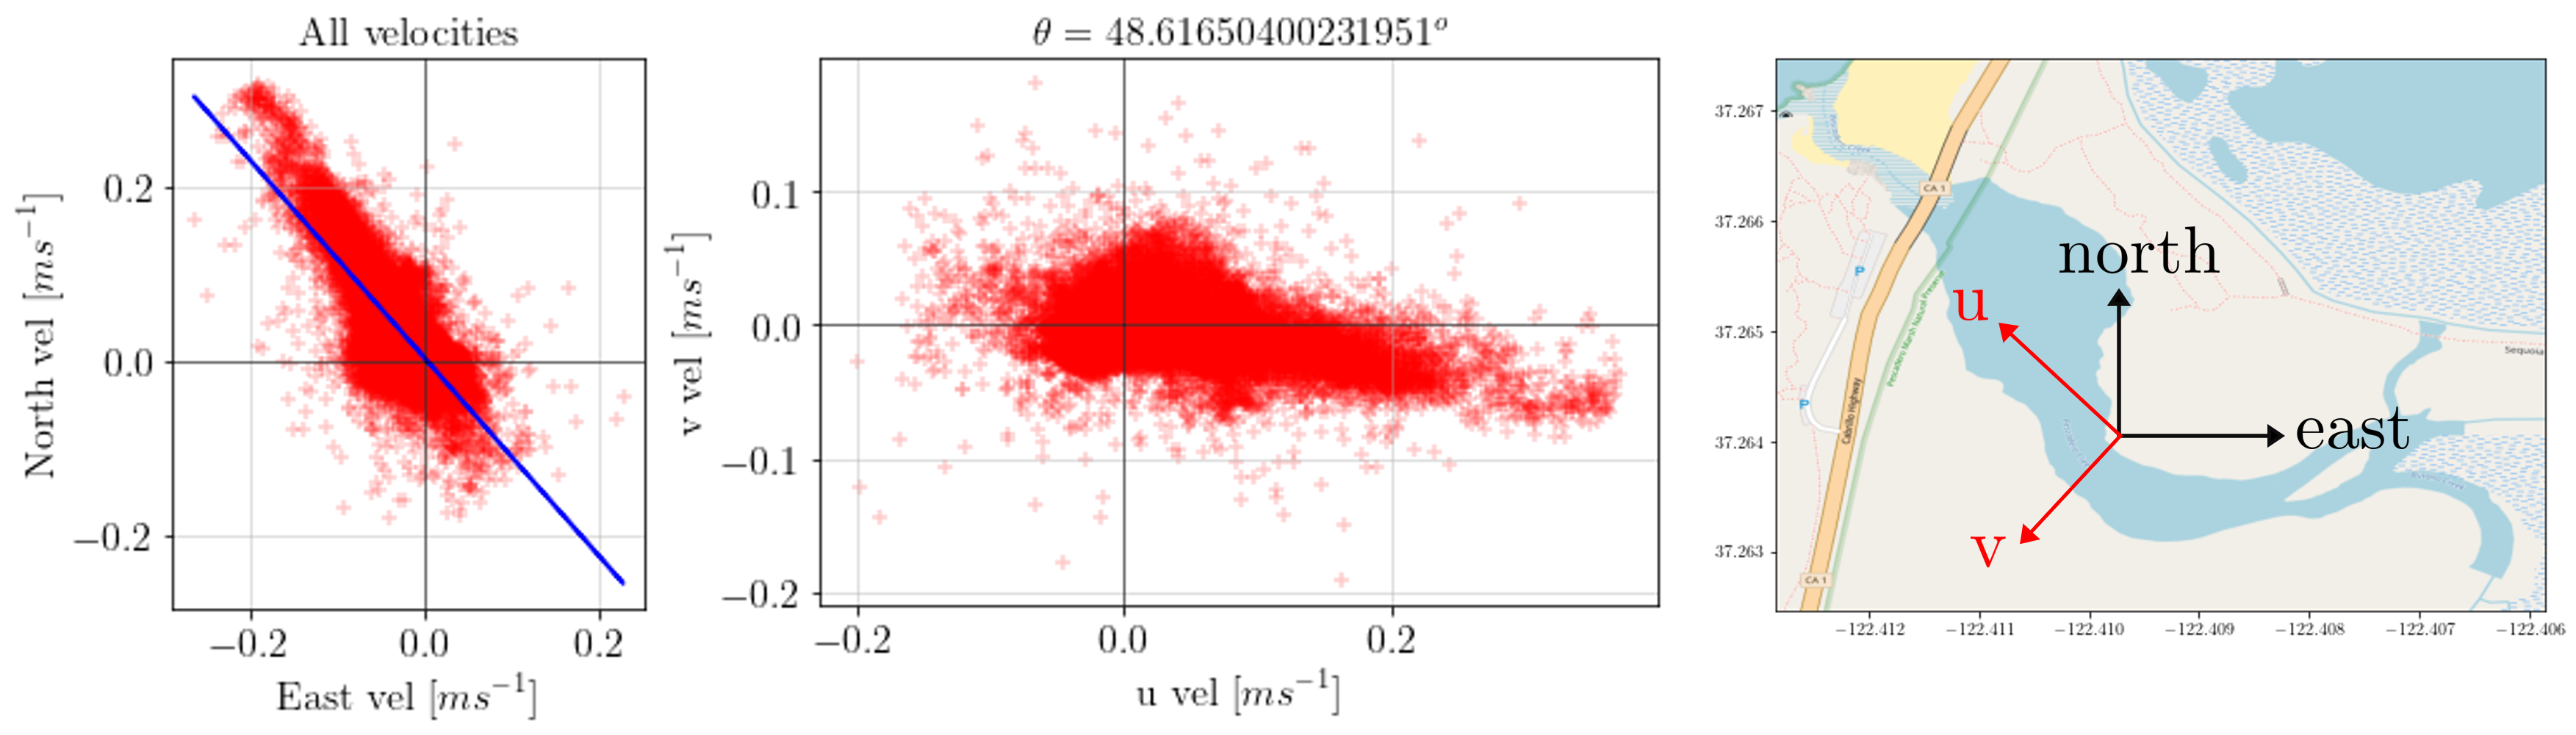
\includegraphics[width=\textwidth]{Imagenes/rotacion.png}
    \caption{Speed data plotted in North-East and $u-v$ coordinates, and a map of Pescadero signaling the coordinates.}
    \label{fig:rotacion}
\end{figure}

ADCP data were averaged every 5 minutes to take off high-frequency signals. However, CTD data at the same location (DC) was not measured at the same depth due to bathymetry, thus we estimated the difference between both and adjusted the first cell to 0.91 m above the bottom of the estuary. \\

\subsubsection{Wind stress}

Wind velocity data were also axis-rotated to the principal coordinates of the estuary currents, with an angle of $48.6^o$. Also, we calculated the wind shear stress above the surface using the equation from \cite{read2011derivation}): 

\begin{equation}
    \tau=\rho_{air} C_D U_{10}^2
    \label{eq: tau}
\end{equation}

Where $\rho_{air}$ is the specific weight of air (1.2 $kg/m^3$), $C_D$ is the drag coefficient and was defined by \cite{large1981open} at 0.0012 for wind velocities between 4 and 11 m/s, and considering that the collected speeds are smaller than 11 m/s and the results are not sensitive to $C_D$ it was set as 0.0012. $U_{10}$ is the adjusted wind speed at 10 meters high, and it was obtained by: 

\begin{equation}
    U_{10}^2=U_z*(1-\frac{C_D}{\kappa}*\ln{\frac{10}{z}})^{-1}
    \label{eq: adjvel}
\end{equation}

with $\kappa=0.4$ as the Von Karmann coefficient and z = 3 m.\\

To study the response of the stratified layers to a wind impulse and identify the upwelling we used the Wedderburn number \citep{Shintani2010}:

\begin{equation}
    W=\frac{g'*h_1^2}{L*u_*^2}
    \label{eq: wed}
\end{equation}

where we estimated $h_1$ as the 30\% of the DC's total depth, L as 392 m, and for $u_*$ and g' we used:

\begin{equation}
    g'=\frac{\rho_{bottom}-\rho_{surface}}{\rho_{surface}}*g
    \label{eq: redg}
\end{equation}

\begin{equation}
    u_*^2=\frac{\tau_w}{\rho_{surface}}
    \label{eq: ustar}
\end{equation}


To analyze the relationship between wind stress and density we standardized and normalized the signals and applied cross-correlation. Cross-correlation between wind stress and density signals is used to find the time lag (phasing) between both and their level of correlation along the locations (propagation) measured in the estuary. Also, we can compare the results to the response tilt time that can be considered as $1/4$ of the internal wave period $T_1$ \citep{stevens1996initial}: 

\begin{equation}
    T_1=\frac{2L}{\sqrt{(\frac{\epsilon g h_1 h_2}{h_1 + h_2})}}
    \label{eq: period}
\end{equation}

\subsubsection{Water level}

To analyze what was happening on the surface, a frequency spectral analysis was carried out in order to identify the most important processes that affect the water level. First, \cite{welch1967use} method was applied to reduce the data noise and there was applied a detrend. Finally, the signal was multiplied by a quadratic window to obtain much clearer data and then apply the frequency spectral analysis. \\

To complement this information, an analysis of the wavelet transform was carried out using the Python package PyWavelets \citep{lee2019pywavelets}. The one-dimensional continuous wavelet transform was applied to the DC surface height data using the first-order Gaussian derivative family for a period range between 10 s and 2.8 min, we limited the frequencies to highlight what is important. This, in order to identify important events and other external phenomena, such as a wave overtopping the sandbar due to high tide. This analysis delivers coefficients that are a function of scale and position and that serve as a scalogram to visualize the wavelet.\\

To carry out a more detailed visual analysis, the standardized heights were obtained at the NM and DC points, where the difference between their real value and their average was obtained, in order to compare the results of both on the same scale. In addition, the difference between the two was calculated and amplified by 10 to exaggerate its trend and observe it more clearly.\\

All the mentioned data were plotted according to local time, to analyze visually considering the factors that affect day and night as temperature and wind. Abrupt decreases in water level that were proceeded by a slow increase in the estuarine water level without tidal influence were defined as mouth openings and when tidal energy is not visible at the water level there is a mouth closure. We observed that the inlet opened twice and each time there are abrupt density changes in the water column.  

\end{document}